\documentclass{article}
\usepackage[utf8]{inputenc}
\usepackage{amsmath}
\usepackage{caption}
\usepackage{subcaption}

\title{Weekly Report}
\author{Junior Team }
\date{June 2020}

\usepackage{natbib}
\usepackage{graphicx}

\begin{document}

\maketitle

\section*{IRB Data Analysis}
Once we had the IRB model set up and could optimize over $P_t$, $P_n$, and the maximum width, our goal was to begin to identify trends in the data.

\section{Normal and Tangential Impulses}
The first interesting correlation we found was between the tangential impulse ($P_t$) and the optimal patch width, which can also be interpreted as the moment applied due to the patch width.


\begin{figure}[h!]
\centering
\caption{Tangential Impulse vs Optimal Width}
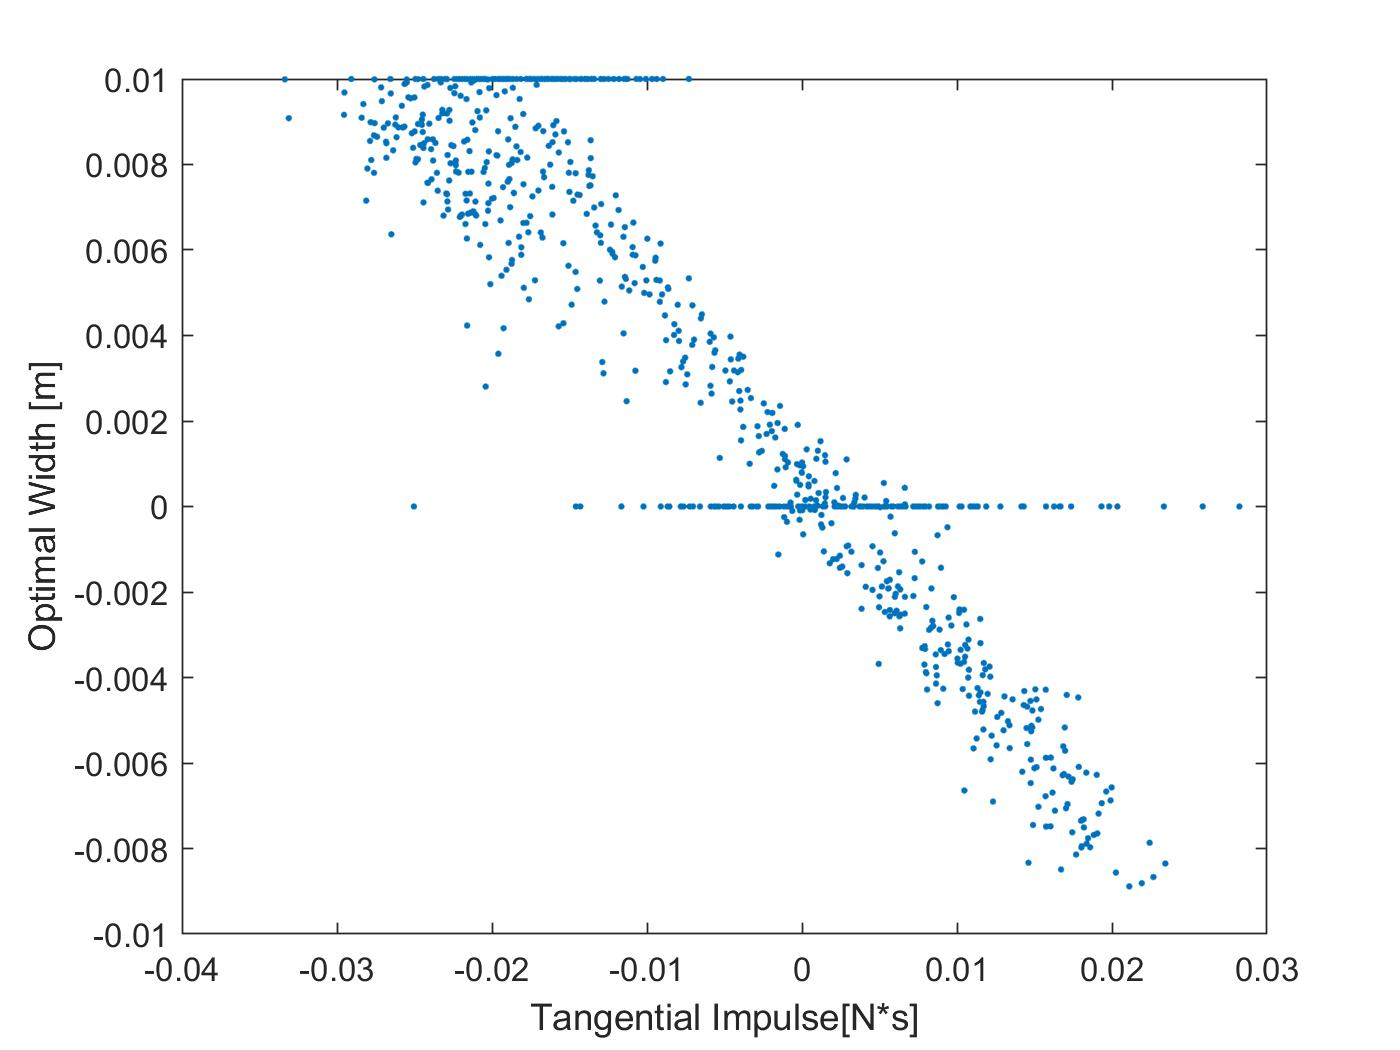
\includegraphics[scale=0.2]{tanImpulse}
\label{fig:tanImpulse}
\end{figure}

\noindent In the figure above, the constraint $\mbox{width} \leq 1 \mbox{cm}$ was used for 1000 different impacts. The correlation coefficient between $P_t$ and width was $ -0.9283$. \\

\noindent  When examining normal impulse ($P_n$) we did not find a clear linear trend, however there seemed to be an impulse threshold below which the optimal width was only zero. From this, we hypothesized that perhaps, those cases to the left of the threshold were below a certain energy threshold, or were lower energy impacts. This would lead to a smaller increase in angular velocity after impact, and less energy in the restitution phase. As a consequence, a patch width which creates a moment and greatly increases the angular velocity ($\dot\theta$) would not be optimal.\\

\noindent To test this hypothesis, we plotted pre- and post-impact kinetic energy versus the optimal patch width. The plots seem to disprove the idea that there is any relationship between zero patch width being optimal and a lower energy collision. 

\begin{figure}[ht]
    \caption{Kinetic Energy Analysis}
    \centering
    \begin{subfigure}[b]{0.45\linewidth}
        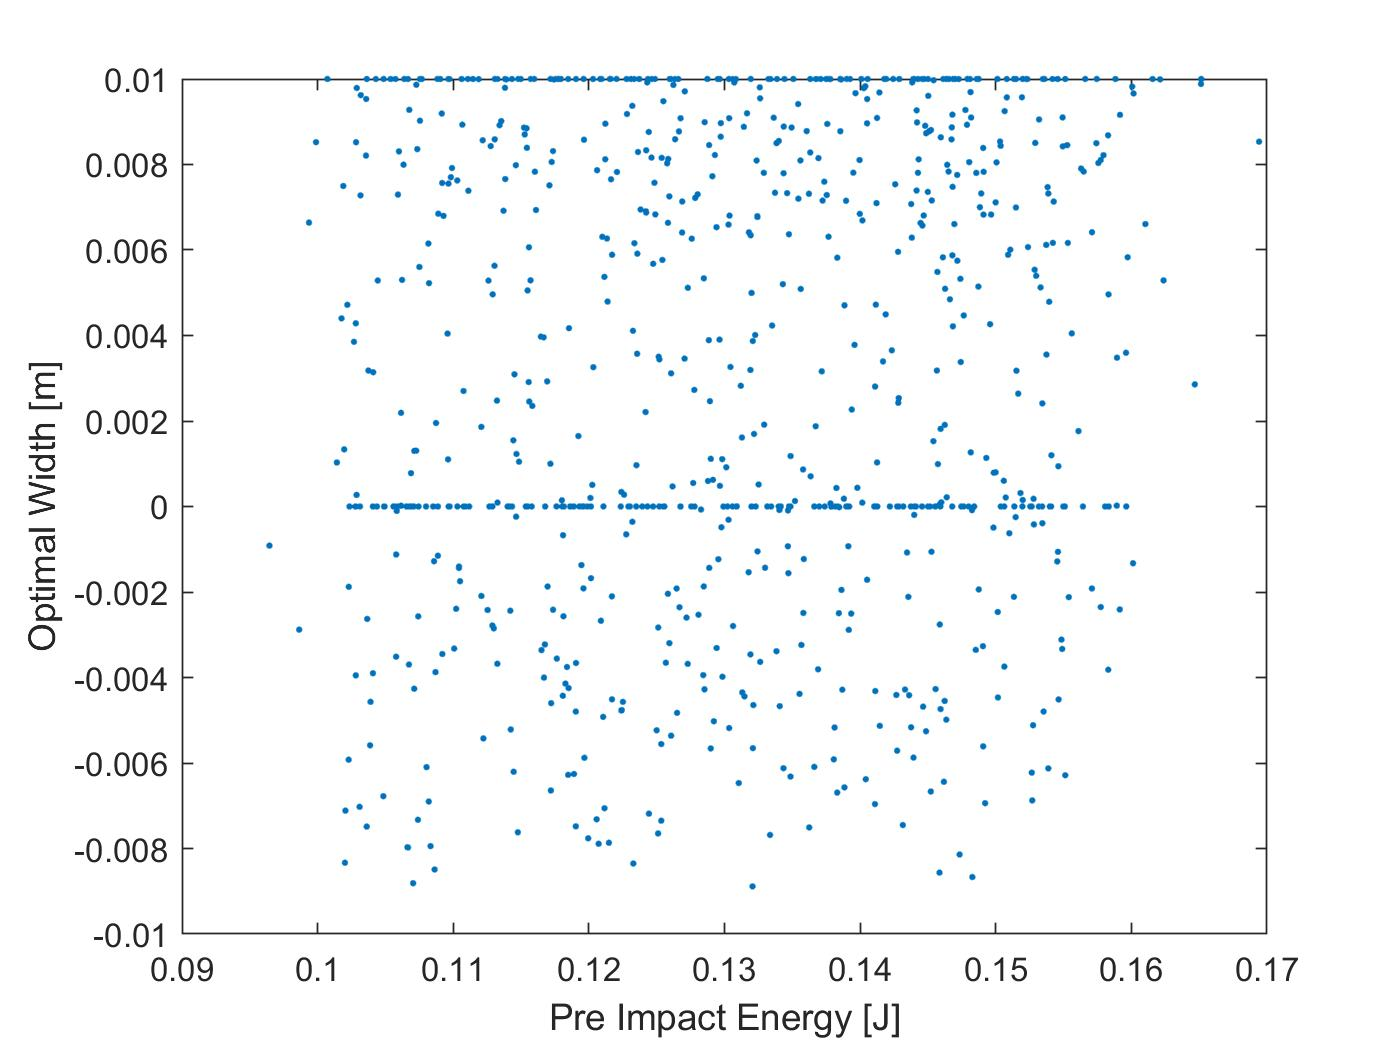
\includegraphics[scale=0.12]{preImpactEnergy.jpg}
        \caption{Pre Impact KE}
        \label{fig:preKE}
    \end{subfigure}
    \quad
    \begin{subfigure}[b]{0.45\linewidth}
       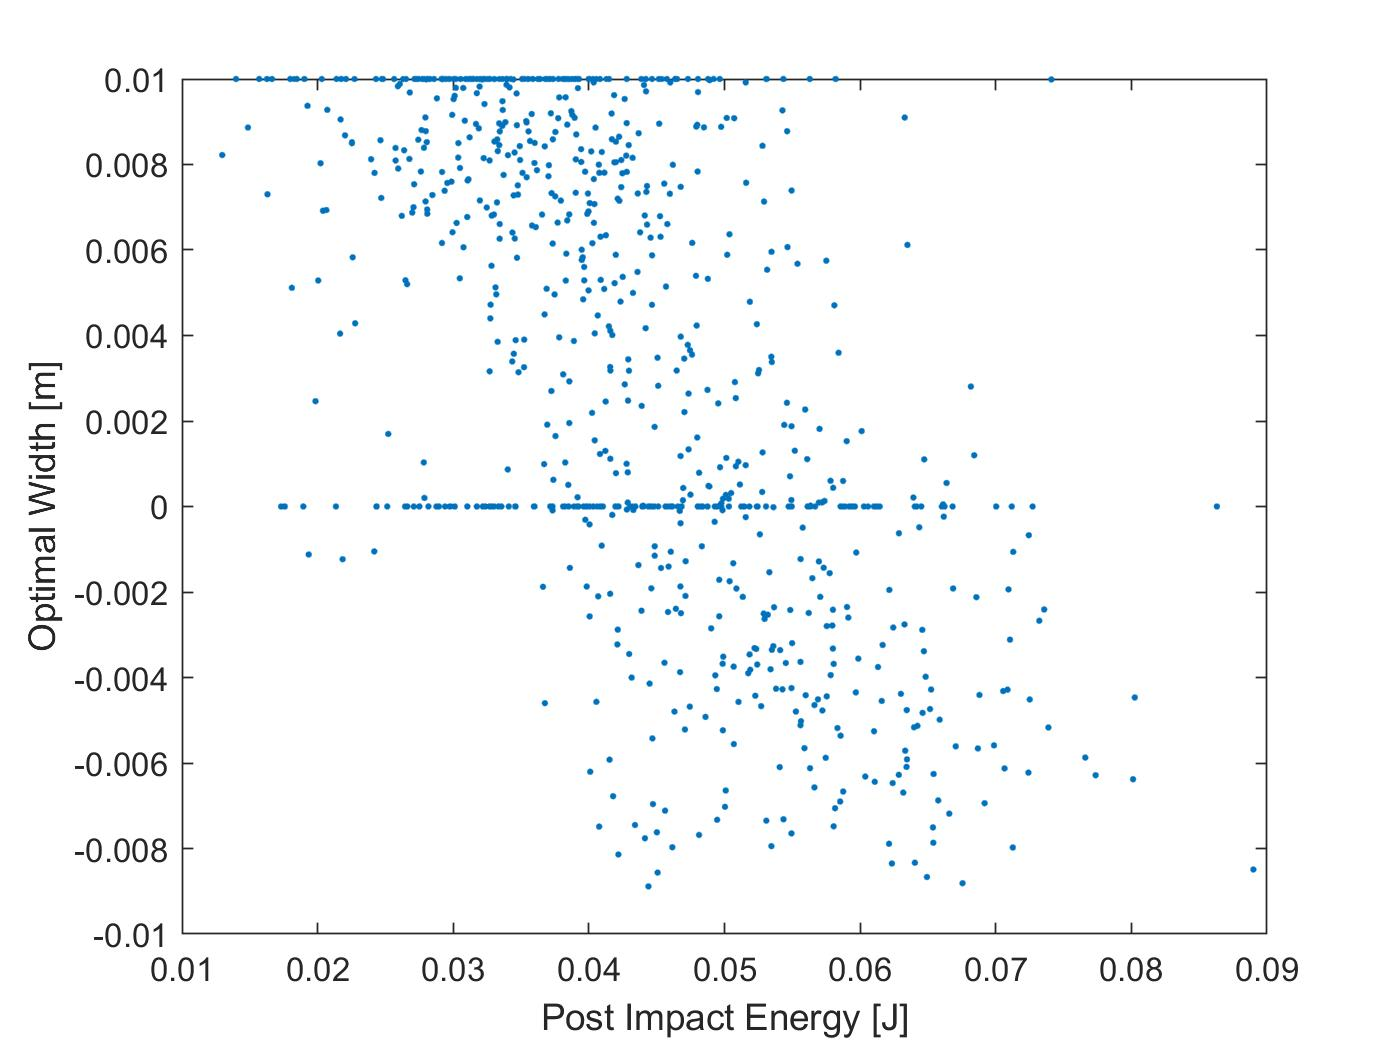
\includegraphics[scale=0.12]{postImpactEnergy.jpg}
        \caption{Post Impact KE}
        \label{fig:postKE}
    \end{subfigure}
\end{figure}

\noindent Additionally, we took a look at the correlation between the net moment and impulses generated from the impact. When inspecting the normal impulse, we found no correlation between the normal impulse and the net moment generated by the ellipse. This is expected, since the configuration of the ellipse as it contacts the surface can be varied greatly, so there should be no definite correlation if the trajectory of the ellipse is not meant to be uniform. \\

\noindent On the other hand, when inspecting the tangential impulse of the ellipse, we find an interesting scatter plot that illustrates a negative correlation between net moment and tangential impulse. Since we assume that the tangential impulse mostly consists of frictional forces and we know that friction tends to oppose motion, we would expect the tangential impulse to be negative when the ellipse has a positive rotation and vice versa. Hence the negative correlation which can be depicted in Fig \ref{fig:tanImpulse2}.


\begin{figure}[ht]
  \begin{subfigure}[b]{0.4\linewidth}
    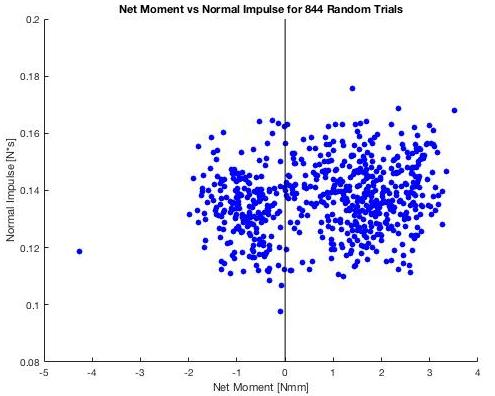
\includegraphics[scale=0.35]{netMomentvsNormImpulse.jpg}
    \caption{Normal Impulse}
    \label{fig:normImpulse}
  \end{subfigure}
  \hfill
  \begin{subfigure}[b]{0.4\linewidth}
    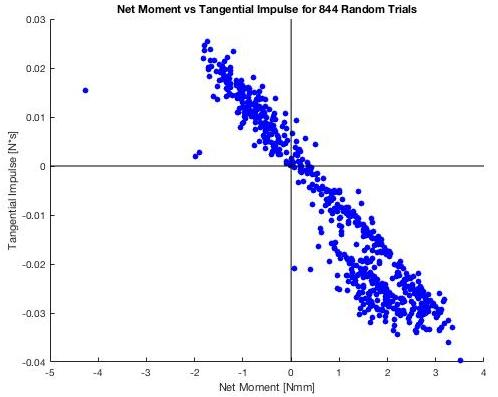
\includegraphics[scale=0.35]{netMomentvsTanImpulse.jpg}
    \caption{Tangential Impulse}
    \label{fig:tanImpulse2}
  \end{subfigure}
  \caption{Impulse vs Net Moment}
\end{figure}

\newpage
\section{Pre-Impact Angle}
The next thing we chose to explore was the relationship between the pre-impact angle ($\theta^+$) and the optimal width. After a plot with a clear trend whose shape resembled an X and Dr. Posa's recommendation, we adjusted the angle transformation to get a cleaner range of angles (wrapped from [$-\pi, \pi$]). We then found another interesting correlation, when the pre-impact angle was plotted with the optimal width, the curve resembled a sin curve. 

\begin{figure}[h!]
\centering
\caption{Pre-Impact Angle vs. Optimal Width}
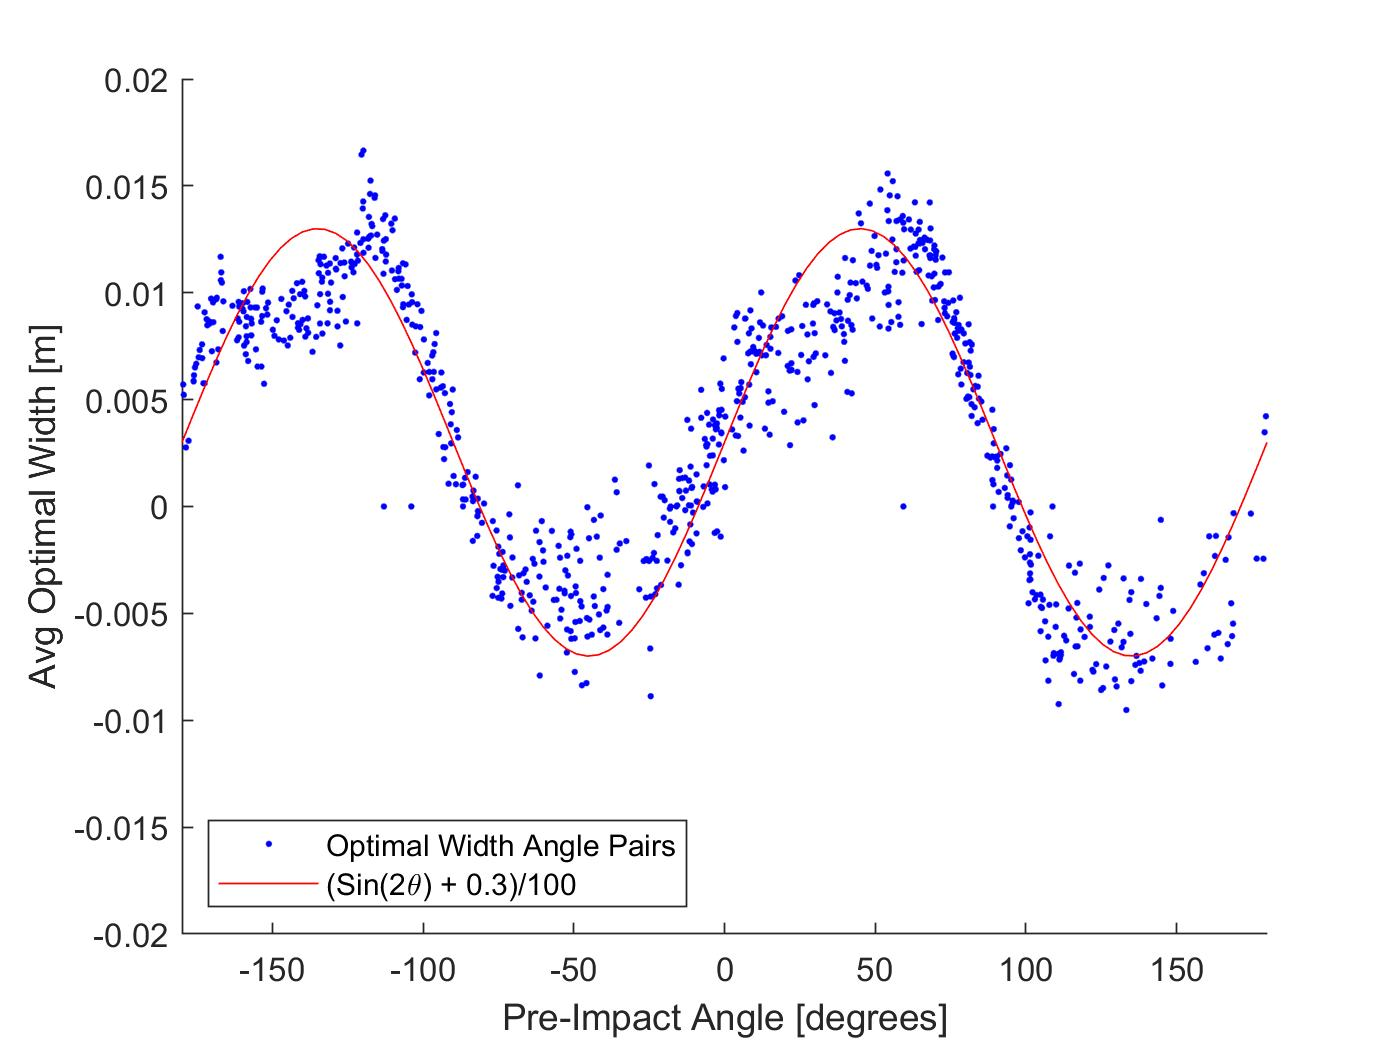
\includegraphics[scale=0.2]{preImpactAngle}
\label{fig:preAngle}
\end{figure}

\noindent The red curve Width $= \frac{1}{100}(sin(2\theta)+0.3)$ clearly correlates with the data. The next thing we checked was whether there was a similar relationship with angular velocity (either $\dot\theta^+$ or $\dot\theta^-$), but there appeared to be nothing. \\

\noindent Interestingly, when we plotted error vs. pre-impact angle for the AP Poisson model and the change in rotational velocity vs. pre-impact angle for the IRB model, the plots also followed a $sin(2\theta)$ trend. \\

\noindent We wanted to explore whether the width depended on the moment arms (Tangential moment arm: vertical distance from the contact point to the COM, normal moment arm: horizontal distance from the contact point to the COM). \\

\noindent The following figures were made without any sort of optimization or considering any impulses. These are just geometric relationships that occur because of the elliptical shape of the object. Whenever the optimal width graphs are mentioned, Figure \ref{fig:preAngle} of Optimal width vs Angle is referenced. \\

\noindent Figure \ref{fig:TanMomentArmVsAngle} shows the relation between the orientation of the ellipse and the tangential moment arm. It shows how that the optimal width is at its max when the tangential moment arm is at its minimum and vice versa, since the optimal width takes the form of a sine wave and the tangential moment arm takes the form of a flipped cosine wave. They both have the same frequency, y-offset, and scaling. The only difference is the amplitude. 

\noindent Figure \ref{fig:NormMomentArmVsAngle} shows the relation between the orientation of the ellipse and the normal moment arm. It shows that the optimal width and the normal moment arm are \textbf{\textit{identical}} in every way, except for the y offset and the reflection of the sine graph of the normal moment arm on the x-axis. This means that there is a direct correlation between the horizontal distance between the contact point and the COM, and the optimal width to account for the rotational impulse.

\begin{figure}[ht]
  \begin{subfigure}[b]{0.4\linewidth}
    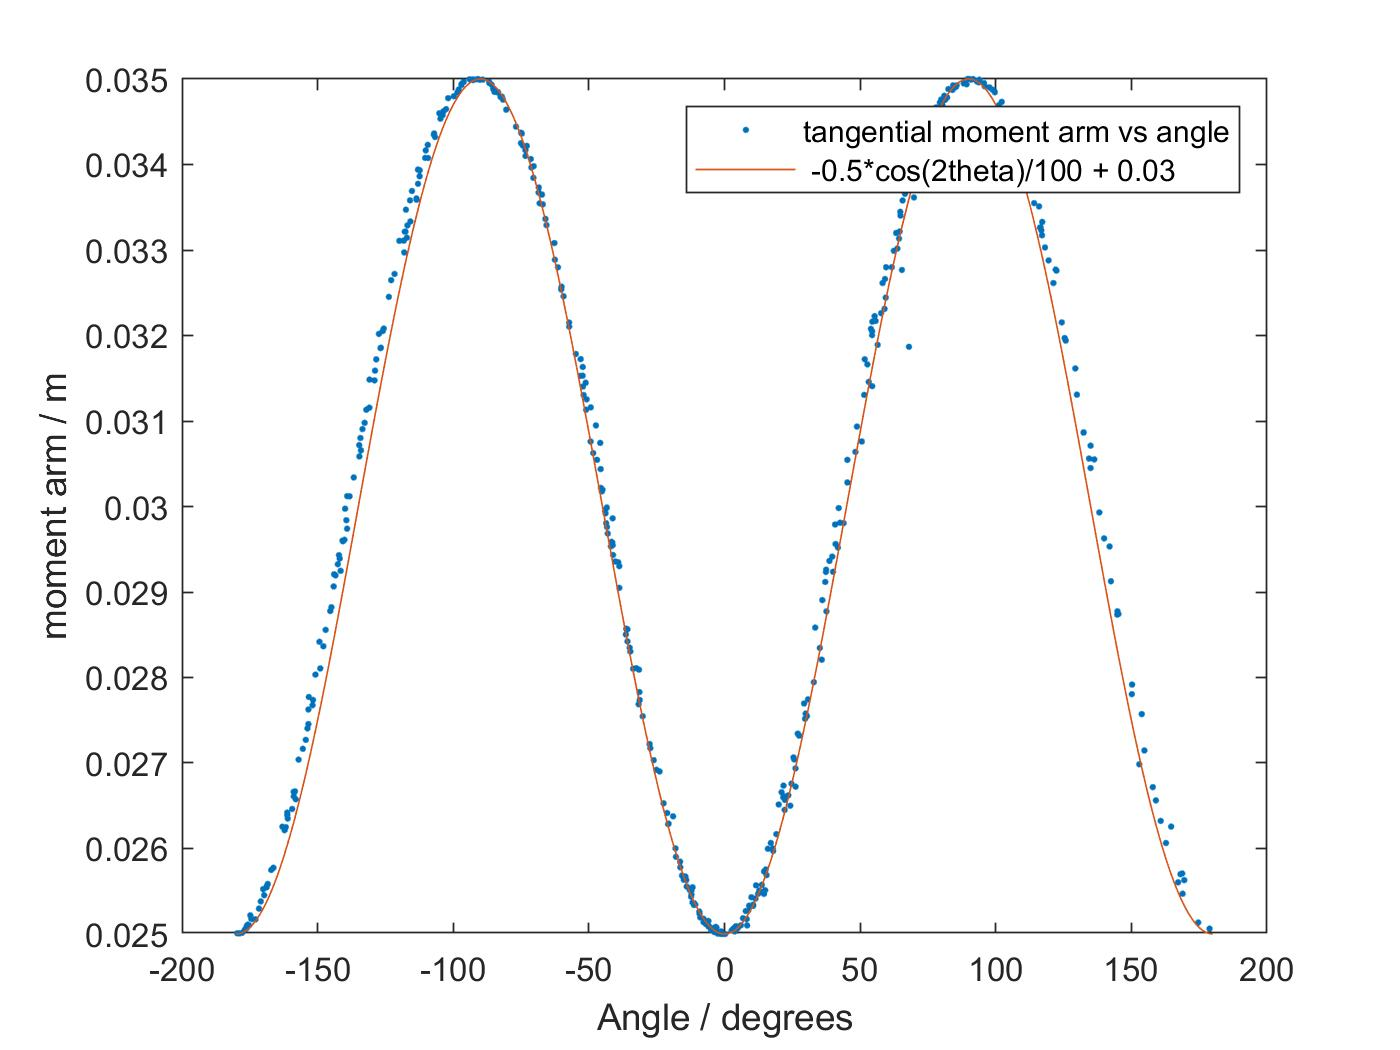
\includegraphics[scale=0.14]{TanMomentArmVsAngle.jpg}
    \caption{ Tangential Moment Arm}
    \label{fig:TanMomentArmVsAngle}
  \end{subfigure}
  \hfill
  \begin{subfigure}[b]{0.4\linewidth}
    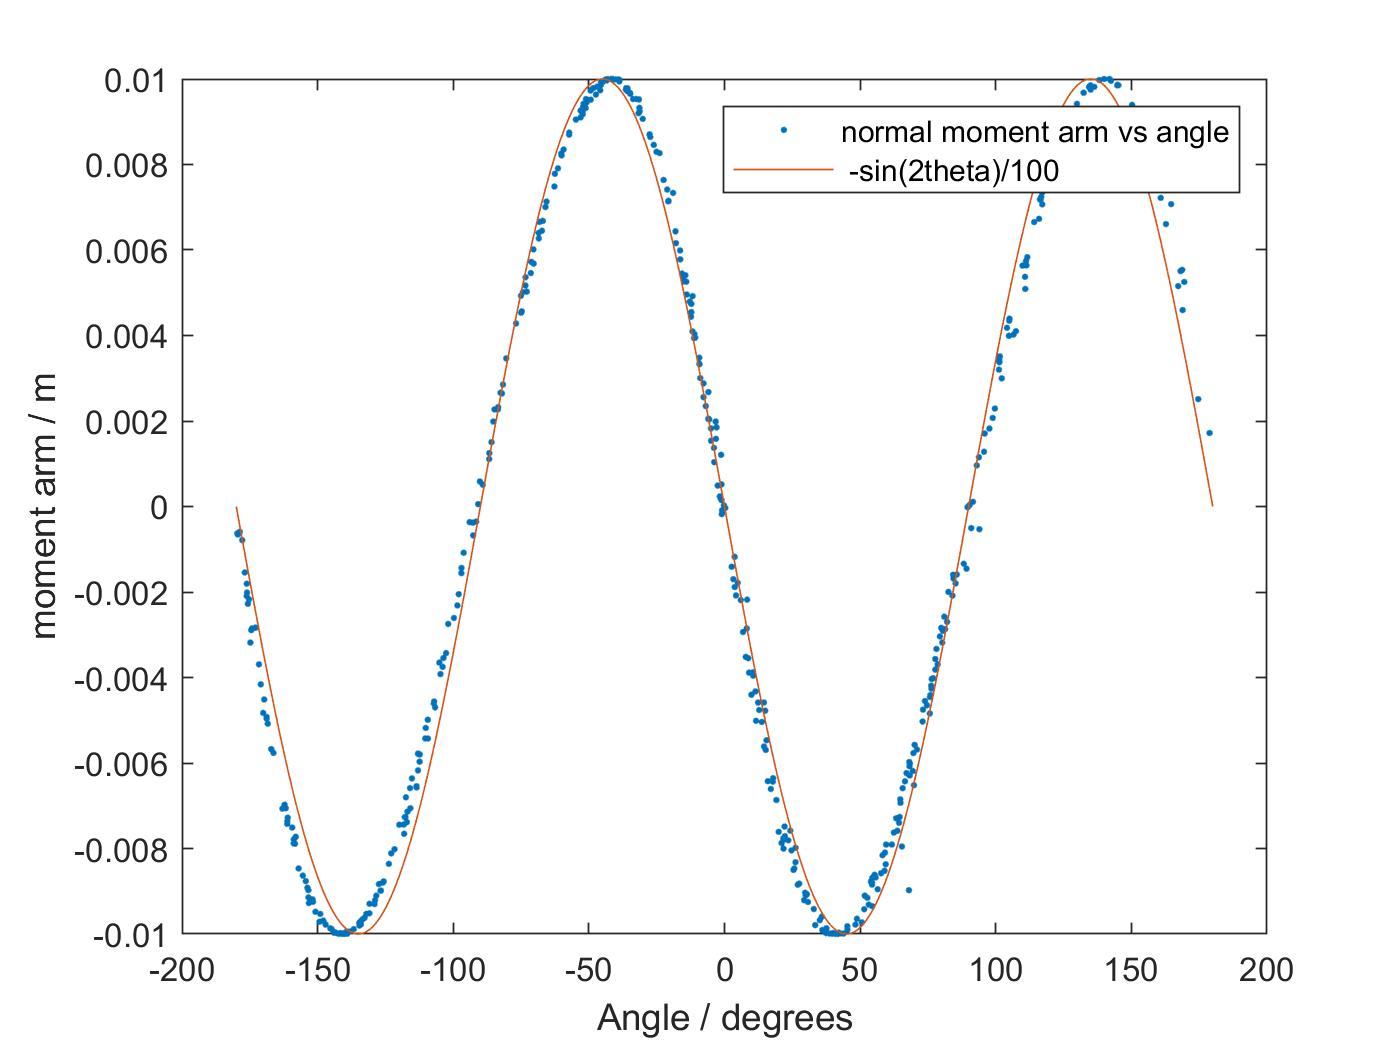
\includegraphics[scale=0.14]{NormMomentArmVsAngle.jpg}
    \caption{Normal Moment Arm}
    \label{fig:NormMomentArmVsAngle}
  \end{subfigure}
  \caption{Moment Arms vs Angle}
\end{figure}

\noindent These relations agree with our predictions and reason.

\section{Moment and Patch Size}
\noindent Initially, we investigated patch size by taking the absolute value of moment. With this, we would see a plot fairly symmetric about $x = 0$ which makes sense since extending the patch from either direction of the center of the contact point should theoretically yield moments equal in magnitude but opposite in sign. However, when we remove this restriction, we can see a linear relationship between net moment and width (Fig \ref{fig:momentPSize}). Dr.\ Posa believed that all of this was pointing towards the idea that error and net moment are correlated, and predicted moment is essentially off by a linear factor:
\begin{align}
    M_{actual} = k * M_{predicted}
\end{align}

\begin{figure}[h!]
\centering
\caption{Net Moment vs. Optimal Patch Size}
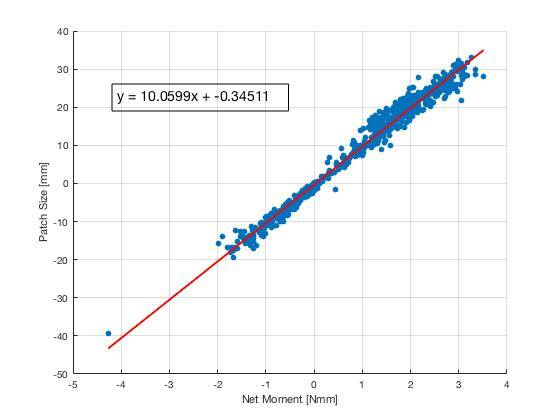
\includegraphics[scale=0.55]{momentPSize}
\label{fig:momentPSize}
\end{figure}

\begin{align}
    \mbox{Best Fit Line: } width = 10.06 * M_{net} - 0.0345
\end{align}
\begin{center}
    Where width and the net moment match the units from the axes in Fig \ref{fig:momentPSize}.
\end{center}

\newpage

\section{Clumping and Convexity}
When we were investigating different potential correlations we began to notice clumping around a patch width of 0 (Fig \ref{fig:tanImpulse}, Fig \ref{fig:preKE}, Fig \ref{fig:postKE}) when we capped the maximum width. For the optimal patch width to be around zero for a given trial when the width is capped below the optimal width, but then have a nonzero optimal width when the range is increased means our solutions were non-convex. This goes against expectations for this sort of problem.To look more closely into why the clumping was occurring, we made fixed width vs error plots for different trials. The shapes of the graphs however, did not give us much insight on why we found clumping, since they seemed to point towards a convex solution. 

\begin{figure}[ht]
  \centering
  \caption{Set Width vs Error Plots for Individual Trials}
  \begin{subfigure}[b]{0.4\linewidth}
    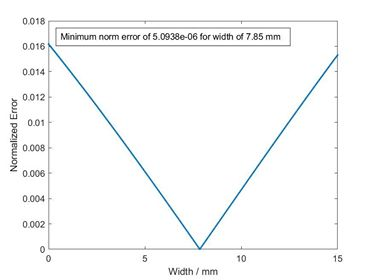
\includegraphics[scale=0.4]{Nat1.jpg}
    \caption{Trial 8}
    \label{fig:cov1}
  \end{subfigure}
  \begin{subfigure}[b]{0.4\linewidth}
    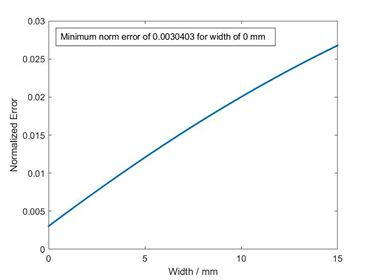
\includegraphics[scale=0.4]{Nat2.jpg}
    \caption{Trial 31}
    \label{fig:cov2}
  \end{subfigure}
\end{figure}

\noindent This is something we will continue to investigate, but for now we will stick to not capping the width at the previously used $1cm$ since we know nearly all of the clumping can be avoided if the cap is raised just half a centimeter to $width_{max} = 1.5cm$.

\newpage

\section{AP Poisson and Wang Mason}
Another thing we did this week was see if we could replicate some of our findings from the IRB model in the two models we had previously worked on and whether we would see similar trends. For the Wang Mason model, we checked for a $x_1$ position we could apply the impulsive forces to minimize error that was within 30\% of it's original value. The plots involving tangential or normal impulse vs. moment matched nicely with those from the IRB model (Fig \ref{fig:normImpulse}, Fig \ref{fig:tanImpulse2}). \\

\noindent A similar approach was taking with the AP Poisson model, where the $x_1$ position was shifted to add an additional moment, also within 30\% of the original value. The tangential and normal impulse plots resembled both Wang and IRB but were not quite as similar. We did observe the same trend between error and pre-impact angle:

\begin{figure}[h!]
\centering
\caption{Error vs Pre-Impact Angle (AP Poisson)}
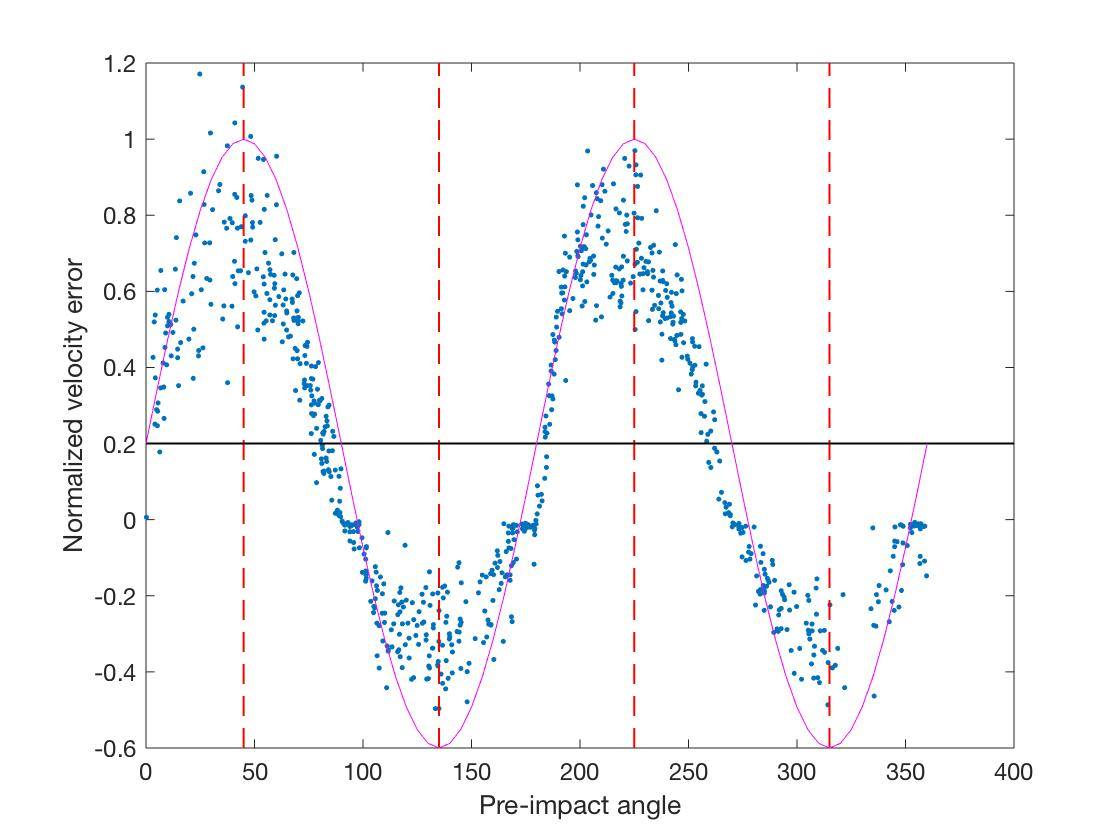
\includegraphics[scale=0.25]{andy1}
\label{fig:andy1}
\end{figure}

\noindent The figure shows how the normalized velocity error follows a similar $sin(2\theta)$ trend to what was observed in the IRB model.


\end{document}
